\documentclass[11pt]{article}
\usepackage[margin=1in]{geometry}
\usepackage{amsmath,amssymb,amsthm}
\usepackage{boldtensors}
% boldtensors declares the symbol font `cmbboard` from the bbold family, which
% is not present in every TeX installation (it aborts at the start of math
% mode). Redirect it to the always-available AMS `msb` family; the `"`-syntax
% that would actually render a cmbboard glyph is unused here, so this only
% removes the missing-font dependency.
\DeclareSymbolFont{cmbboard}{U}{msb}{m}{n}
\usepackage{hyperref}
\usepackage{booktabs}
\usepackage{enumitem}
\usepackage{graphicx}

\newcommand{\dd}{\mathrm{d}}
\newcommand{\Real}{\mathbb{R}}
\newcommand{\norm}[1]{\lVert #1 \rVert}
\newcommand{\code}[1]{\texttt{#1}}
\newcommand{\jump}[1]{[\![#1]\!]}
\emergencystretch=3em

\title{Diagnosis: Interface Energy Loss of the Impedance-Overlap Schwarz\\
Coupling on Nonconforming Meshes, and an Energy-Consistent Redesign}
\author{Alejandro Mota}

\begin{document}
\maketitle

\begin{abstract}
A $4\times3\times3$ parametric study of the impedance-overlap Schwarz coupling
on the bent-cantilever release problem (integrator pairs II/IE/EI/EE $\times$
overlap widths $\{0.0508, 0.0254, 0.0127\}$\,m $\times$ mesh ratios
$\{1{:}1, 3{:}4, 1{:}2\}$, $1$\,ms at $\Delta t = 10^{-6}$\,s) shows the
partition-of-unity energy conserved to $0.1\%$ on conforming meshes but losing
$28$--$71\%$ --- and in one case \emph{gaining} $12\%$ --- on nonconforming
ones. A follow-up $108$-run sweep over mesh ratios $1{:}1.0$--$1{:}0.2$
(Sec.~\ref{sec:ratiosweep}) shows the gain is generic, not exceptional: even
with variational transfer, mild coarsening injects up to $+45\%$, one
configuration pumps the beam to $+275\%$ of its initial energy, and the sign
of the drift flips between adjacent mesh ratios. Channel-resolved interface-work instrumentation and an impedance-scale
sweep identify the cause: the impedance dashpot $~Z(\dot{~u}_p - \dot{~u})$
acts on an interface velocity jump that cannot vanish at Schwarz convergence
when the two trace spaces differ, and because the two subdomains transfer
partner data through \emph{independent, non-adjoint} interpolations, the
dashpot work is not even sign-definite. The optimized-Schwarz, multi-time-step,
and discontinuous-Galerkin literatures converge on the same two structural
requirements for an energy-consistent coupling: (i) the kinematic transfer and
the force transfer between the two sides must be $L^2$-adjoints through a
single variational cross-mass matrix, which makes the interface power telescope to
a sign-definite dashpot on the common-space jump plus a \emph{conservative}
spring term; and (ii) the dashpot must act only on content both trace spaces
can represent, so that it vanishes at Schwarz convergence instead of
persistently absorbing unrepresentable fine-scale content. These requirements
are implementable only on the \emph{nonoverlap} impedance variant (single
shared interface), where --- together with a dynamically consistent
d'Alembert interface traction and an IMEX treatment of the interface rows
for explicit subdomains --- they are now implemented and validated:
implicit--implicit drift improves from $-9.6\%$ to $-0.03\%$ on conforming
and mildly nonconforming meshes, the conforming explicit--explicit
trajectory matches the monodomain explicit run to $0.35\%$ pointwise, and
every injection pathology disappears (Sec.~\ref{sec:nonoverlap}). Under
subcycling, two infrastructure defects that had silently reduced the
multi-time-step exchange to end-sampled partner data are fixed --- genuine
Gravouil--Combescure interpolation then halves the excess dissipation at
strong mesh contrast --- and the Prakash--Hjelmstad exact-telescoping
refinement is measured to be structurally incompatible with a partitioned
exchange: its work-conjugate data are either lagged (over-dissipative) or
anticipatory (unstable), so exact subcycled telescoping requires a direct
interface solve (Sec.~\ref{sec:subcycle}). A ten-fold horizon extension
($10$\,ms, all $151$ configurations, Sec.~\ref{sec:tenms}) sharpens the
verdict: the overlap family is long-horizon \emph{unstable} almost
everywhere ($74$ of $108$ runs die of element inversion after exponential
growth; only conforming II survives healthy), while the paired nonoverlap
coupling never injects but compounds its dissipation at strong contrast,
develops a failure window at mild non-nested mesh ratios, and saturates
with undamped grid-frequency content when both members are explicit at
$\mathrm{CFL}=1$. Finally, a controller-step sweep exposes --- and fixes ---
a defect of the Schwarz relaxation machinery itself: with controller stops
larger than a subdomain's time step, the per-pair relaxation state blended
iterates across \emph{time}, a causal low-pass on the exchanged traction
that shifted the converged fixed point (up to $-88\%$ at ten substeps per
stop on the conforming pair, and energy injection under Aitken
acceleration). The state is now keyed per substep time slot, restoring
windowed $\equiv$ same-step to Schwarz truncation; Aitken acceleration is
restricted to single-slot stops after every windowed variant measured
worse than a fixed relaxation parameter (Sec.~\ref{sec:windowed}). This
note records the evidence, the theory, the phased redesign, and the
validated fixes.
\end{abstract}

\section{Observed behavior}
\label{sec:observed}

The benchmark is the bent 3D cantilever released from a parabolic initial
displacement, split lengthwise into clamped and free subdomains that overlap,
coupled by the impedance-overlap transmission condition
\begin{equation}
  ~t \;=\; ~t_p \;+\; ~Z\,(\dot{~u}_p - \dot{~u}) \;+\; \alpha\,(~u_p - ~u),
  \qquad
  ~Z = Z_p\,~n\otimes~n + Z_s\,(~I - ~n\otimes~n),
  \label{eq:tc}
\end{equation}
with $Z_p = \rho c_p$, $Z_s = \rho c_s$ of the partner material
(Lysmer--Kuhlemeyer split), $\alpha = 0$ throughout this study, and subscript
$p$ denoting partner fields evaluated at this subdomain's Schwarz boundary.
Energy is the Arlequin partition-of-unity total (overlap counted once),
normalized by each run's own $E(0) \approx 1506$\,J.

Drift $E(1\,\mathrm{ms})/E(0) - 1$, in percent, pointwise transfer:

\begin{center}
\begin{tabular}{llrrrr}
\toprule
overlap & ratio & II & IE & EI & EE \\
\midrule
0.0508 (max) & 1:1 & $-0.07$ & $-8.9$ & $-0.2$ & $+8.7$ \\
             & 3:4 & $+1.1$  & $-8.7$ & $-0.9$ & $-12.0$ \\
             & 1:2 & $+12.5$ & $-26.5$ & $-53.8$ & $-57.7$ \\
0.0254 (\textonehalf) & 1:1 & $-0.07$ & $+5.0$ & $-0.4$ & $+10.2$ \\
             & 3:4 & $-28.4$ & $-6.0$ & $-22.3$ & $-13.9$ \\
             & 1:2 & $-17.3$ & $-18.5$ & $-58.9$ & $-45.7$ \\
0.0127 (\textonequarter) & 1:1 & $-0.02$ & $-15.7$ & $-6.1$ & $+3.6$ \\
             & 3:4 & $-44.5$ & $-40.6$ & $-41.1$ & $-31.4$ \\
             & 1:2 & $-63.8$ & $-64.3$ & $-70.8$ & $-61.9$ \\
\bottomrule
\end{tabular}
\end{center}

Three regimes: (a) conforming ($1{:}1$) implicit-free-subdomain runs conserve
to $\le 0.1\%$ at every overlap; (b) nonconforming runs lose tens of percent,
worse with mesh ratio and with smaller overlap; (c) a minority of cases,
including II at max overlap $1{:}2$, \emph{gain} energy. Variational
(\code{transfer: variational}) rescues the small-overlap losses dramatically
($-44.5 \to -4.4\%$ at \textonequarter/3:4) but regresses elsewhere
($+12.5 \to -50.7\%$ at max/1:2): it improved 17 of 24 nonconforming cases,
mean $|$drift$|$ $33.4 \to 25.4\%$ --- helpful, not structural.

\section{Empirical diagnosis}
\label{sec:diagnosis}

\subsection{Channel-resolved interface work}

The instrumentation (\code{NORMA\_IMPEDANCE\_WORK\_CSV}) decomposes each
subdomain's interface power $P = \sum_i \dot{~u}_i \cdot ~f^{\mathrm{bc}}_i$
into the traction, dashpot, and Robin channels of \eqref{eq:tc}. For the exact
monodomain solution the dashpot and Robin channels vanish identically, so
their work is purely spurious. Integrated over 1\,ms (II runs; work summed
over both subdomains):

\begin{center}
\begin{tabular}{lrrrr}
\toprule
case & $\Delta E$ blended & dashpot work & traction work & jump RMS \\
\midrule
conforming (\textonehalf, 1:1)          & $-1$\,J    & $-1.8$\,J  & $+70$\,J  & $\sim 1$ \\
nonconf.\ \textonehalf, 3:4 (pointwise) & $-428$\,J  & $-586$\,J  & $+92$\,J  & $\sim 20$ \\
nonconf.\ \textonequarter, 3:4 (pointwise) & $-515$\,J & $-877$\,J & $+341$\,J & $\sim 16$ \\
nonconf.\ max, 1:2 (pointwise)          & $+188$\,J  & $\mathbf{+554}$\,J & $-211$\,J & $\sim 80$ \\
nonconf.\ \textonequarter, 3:4 (variational) & $-67$\,J & $-864$\,J & $+780$\,J & $\sim 26$ \\
\bottomrule
\end{tabular}
\end{center}

Three facts follow. First, on conforming meshes the dashpot channel is
negligible ($-1.8$\,J) and the coupling is conservative: the jump
$\dot{~u}_p - \dot{~u}$ closes at Schwarz convergence. Second, on
nonconforming meshes the dashpot channel carries the loss: the jump RMS is an
order of magnitude larger and never closes --- the coarse trace space cannot
represent the fine side's boundary velocity, and the dashpot persistently
absorbs the difference, exactly as a Lysmer--Kuhlemeyer boundary absorbs
outgoing content. Third, and decisively for the mechanism: in the max/1:2 case
the ``dashpot'' does $+554$\,J of \emph{positive} work. A dissipator can never
do positive work; this proves the discrete dashpot term is not a quadratic
form. Because each subdomain interpolates partner fields with its own,
unrelated operator, the two sides' dashpot terms do not pair, and the total is
sign-indefinite.

The variational row explains why variational transfer helps only sometimes: its
dashpot still drains $-864$\,J, but the consistent (characteristic-transfer)
traction returns $+780$\,J. The rescue is an accidental near-cancellation of
two large opposing channels, not a removal of either defect.

\subsection{Impedance-scale sweep}

Scaling both impedances by $s \in \{1, 0.5, 0.25\}$ on the
\textonequarter/3:4 II case (pointwise):

\begin{center}
\begin{tabular}{lccc}
\toprule
impedance scale $s$ & 1.0 & 0.5 & 0.25 \\
\midrule
drift at 1 ms & $-44.5\%$ & $-40.5\%$ & $-29.2\%$ \\
\bottomrule
\end{tabular}
\end{center}

The loss decreases monotonically as the dashpot is weakened --- confirming the
dashpot as the carrier of the loss --- but sublinearly: the dissipated power is
$Z\,\jump{\dot{u}}^2$ and the jump itself grows as the absorber detunes
(reflection increasing as $Z \to 0$), so the product falls more slowly than
$Z$. This is the signature of an absorbing-boundary mechanism rather than of a
fixed damping force, consistent with the channel decomposition above.

\subsection{Control experiment: hard Dirichlet matching}
\label{sec:dbc}

To separate ``defect of the impedance condition'' from ``price of
nonconforming overlap coupling,'' the same nine mesh configurations were run
with the classical Dirichlet-overlap coupling (II), in both transfer flavors
--- pointwise interpolation and the weak (variational $L^2$-projection)
Dirichlet option:

\begin{center}
\begin{tabular}{llrr}
\toprule
overlap & ratio & DBC pointwise & DBC weak \\
\midrule
0.0508 (max) & 1:1 & $+0.05\%$ & --- \\
             & 3:4 & $+5507\%^{*}$ & $+2418\%$ \\
             & 1:2 & $+2765\%^{*}$ & $+5752\%^{*}$ \\
0.0254 (\textonehalf) & 1:1 & $-0.03\%$ & --- \\
             & 3:4 & $+423\%$ & $+749\%$ \\
             & 1:2 & $+5628\%^{*}$ & $+7765\%^{*}$ \\
0.0127 (\textonequarter) & 1:1 & $+0.01\%$ & --- \\
             & 3:4 & $+33\%$ & $+22\%$ \\
             & 1:2 & $+3268\%^{*}$ & $+262\%$ \\
\bottomrule
\end{tabular}\\[2pt]
{\footnotesize $^{*}$ run died (Newton failure) before 1\,ms; drift at last stop.}
\end{center}

Hard matching conserves essentially exactly on conforming meshes and is
\emph{violently unstable} on every nonconforming one --- and the weak
(contraction) transfer does \emph{not} rescue it. Two consequences. First, the
impedance dashpot's dissipation is not merely a defect: it is what
\emph{stabilizes} a coupling that hard kinematic exchange destabilizes; its
magnitude is the energy in the inter-grid disagreement it must continually
absorb. Second, the Dirichlet instability grows with overlap \emph{width}
(opposite to the impedance losses), consistent with a feedback loop between
the two interpolation surfaces through the overlap volume.

\section{Mesh-ratio sweep: injection is generic}
\label{sec:ratiosweep}

An independent, finer-grained parametric study by our intern Lukas reported
significant energy \emph{injection} at mesh ratios the original
$\{1{:}1, 3{:}4, 1{:}2\}$ grid does not sample. The following sweep confirms
and maps it: same beam, release, and symmetric subdomains
$L_{\mathrm{sub}} = (0.254 + \mathrm{ov})/2$; free mesh fixed at
$h = 6.35$\,mm; clamped mesh coarsened to $6.35/r$\,mm for
$r = 1.0, 0.9, \dots, 0.2$ (clamped:free element-size ratio $1{:}r$;
$1{:}0.1$ skipped); all three overlap widths; all four integrator pairs;
variational transfer (now the default) throughout --- $108$ runs. The
$1{:}1.0$ column reproduces the conforming baselines of
Sec.~\ref{sec:observed} to all printed digits, and $1{:}0.5$ reproduces the
earlier variational $1{:}2$ results exactly.

\begin{center}
\small\setlength{\tabcolsep}{3.6pt}
\begin{tabular}{l rrrr rrrr rrrr}
\toprule
& \multicolumn{4}{c}{overlap 0.0508\,m} & \multicolumn{4}{c}{overlap 0.0254\,m}
& \multicolumn{4}{c}{overlap 0.0127\,m} \\
\cmidrule(lr){2-5}\cmidrule(lr){6-9}\cmidrule(lr){10-13}
ratio & II & IE & EI & EE & II & IE & EI & EE & II & IE & EI & EE \\
\midrule
1:1.0 & $-0.1$ & $-8.9$ & $-0.2$ & $+8.7$ & $-0.1$ & $+5.0$ & $-0.4$ & $+10.2$ & $-0.0$ & $-15.7$ & $-6.1$ & $+3.6$ \\
1:0.9 & $+7.6$ & $-11.7$ & $-5.5$ & $+8.5$ & $-4.4$ & $-8.1$ & $+4.4$ & $+9.1$ & $+0.1$ & $-14.8$ & $-1.0$ & $+4.3$ \\
1:0.8 & $\mathbf{+29.8}$ & $-15.3$ & $+5.5$ & $-9.5$ & $+20.4$ & $\mathbf{+45.1}$ & $-2.4$ & $-1.9$ & $-3.1$ & $-20.3$ & $-5.4$ & $+4.7$ \\
1:0.7 & $+19.2$ & $-12.8$ & $+2.7$ & $-11.6$ & $+11.8$ & $-18.6$ & $+0.7$ & $-5.4$ & $+11.1$ & $+7.3$ & $-9.8$ & $-17.9$ \\
1:0.6 & $-61.1$ & $-54.0$ & $-57.7$ & $-40.4$ & $+2.1$ & $-18.6$ & $-63.9$ & $-53.4$ & $-4.5$ & $-34.2$ & $-57.1$ & $-52.7$ \\
1:0.5 & $-50.6$ & $-32.3$ & $-36.4$ & $-56.8$ & $-11.0$ & $-17.6$ & $-55.7$ & $-54.3$ & $-29.2$ & $-54.0$ & $-56.8$ & $-52.0$ \\
1:0.4 & $-12.4$ & $+3.9$ & $-43.1$ & $-53.1$ & $-52.7$ & $-50.2$ & $-57.0$ & $-63.8$ & $-36.6$ & $-52.4$ & $-78.2$ & $-76.2$ \\
1:0.3 & $-65.0$ & $-44.5$ & $-78.3$ & $-57.4$ & $\mathbf{+173.7}$ & $\mathbf{+274.7}$ & $-81.2$ & $-78.8$ & $-30.5$ & $-58.6$ & $-79.5$ & $-79.4$ \\
1:0.2 & $-79.1$ & $-76.8$ & $-80.8$ & $-78.9$ & $-66.5$ & $-66.2$ & $-86.3$ & $-87.4$ & $-22.2$ & $-45.8$ & $-91.2$ & $-90.3$ \\
\bottomrule
\end{tabular}
\end{center}

Three observations sharpen the diagnosis.

\begin{description}[style=unboxed,leftmargin=0pt,itemsep=2pt]
  \item[Injection at mild coarsening is systematic, not exceptional.] The
  implicit-clamped pairs (II, IE) inject at nearly every overlap for ratios
  $1{:}0.9$--$1{:}0.7$: II $+29.8\%$ at max$/1{:}0.8$, IE $+45.1\%$ at
  \textonehalf$/1{:}0.8$, and seven further cells above $+7\%$. This is with
  the variational (contraction) transfer already in place: the contraction
  property bounds the \emph{transfer} but not the sign of the dashpot work,
  confirming that no per-side transfer improvement yields sign-definiteness on
  the two-surface overlap coupling (cf.\ the reframed Phase~1).
  \item[A violent injection resonance.] At \textonehalf$/1{:}0.3$ the coupling
  pumps the beam to $+174\%$ (II) and $+275\%$ (IE) of $E(0)$. The energy
  grows smoothly for ${\sim}0.7$\,ms and saturates near $3$--$4\times E(0)$
  --- steady interface pumping, not a numerical explosion. At this ratio the
  clamped mesh has degenerated to a single-element cross-section (seven
  bricks in total; one element through the thickness from $1{:}0.7$ down), so
  it cannot represent the bending wave at all. Degeneracy alone does not
  decide the outcome, however: the \emph{same} clamped mesh at quarter
  overlap dissipates $-30.5\%$ (II), and the explicit-clamped pairs on the
  identical configuration dissipate $-81\%$. Whether the sign-indefinite
  interface work pumps or absorbs is a property of the mesh \emph{pair} and
  the overlap geometry together.
  \item[The drift is violently non-monotone in the ratio.] At \textonehalf\
  overlap, II moves $-52.7 \to +173.7 \to -66.5\%$ across the three adjacent
  ratios $1{:}0.4 \to 1{:}0.3 \to 1{:}0.2$. There is no usable regime map
  ``mild contrast $=$ small drift'': both the sign and the magnitude of the
  energy defect are extremely sensitive to the discrete mesh pair.
\end{description}

Practically, this closes the question of whether the nonconforming overlap
coupling can be trusted with a drift \emph{budget}: it cannot. The interface
work is sign-indefinite (Sec.~\ref{sec:diagnosis}), and this sweep shows both
signs realized at large amplitude across neighboring points of a smooth
parameter family. Data: \code{ratio-sweep/} in the study bundle.

\section{What the literature says}
\label{sec:theory}

Four independent lines of analysis (all in
\code{\textasciitilde/Downloads/Optimized-Schwarz-Methods}) agree on the
structure of the problem and of its solution.

\subsection{The interface-work pairing identity}

For Newmark-family subdomains coupled by interface tractions, the discrete
energy balance over a step contains the interface term
(Gravouil--Combescure 2001, Eq.~(34); Karimi--Nakshatrala 2014, Eq.~(84))
\begin{equation}
  E_{\mathrm{int}}
  = \sum_{\text{sides }k} \frac{1}{\Delta t_k}\,
    \jump{\dot{~u}_k}^{T} ~C_k^{T}\, \jump{\Lambda_k},
  \label{eq:eint}
\end{equation}
the work of the transmitted tractions through the kinematic jump, each side on
its own grid. It vanishes iff the traction is a \emph{single-valued} field
acting equal-and-opposite on the two sides through \emph{adjoint} trace
operators, with velocity continuity enforced at instants shared by both time
grids. Gravouil--Combescure prove their subcycled coupling makes
$E_{\mathrm{int}} \le 0$ (dissipative, never a source);
Prakash--Hjelmstad restructure the intermediate tractions so it telescopes to
exactly zero. Neither treats spatially nonconforming interfaces; both warn
that breaking the pairing leaves $E_{\mathrm{int}}$ of indefinite sign ---
precisely the $+554$\,J observation.

\subsection{Representability: the converged nonconforming solution}

Gander--Halpern--Nataf (SINUM 2003) analyze discrete Schwarz waveform
relaxation with impedance transmission on nonmatching grids. Their key
statements: the choice $Z = \rho c$ of the \emph{partner} side is the exact
transparent operator in 1D and optimal-in-class generally (\S3, Eq.~(3.10)) ---
so the impedance choice is not the problem; their nonmatching-grid convergence
proof requires the intergrid transfer to be an $L^2$ \emph{contraction}
(projection qualifies, Eq.~(5.24); pointwise interpolation does not); and, for
nonconforming grids, ``the coupled system \emph{defines} the solution when
converged'' (\S5.4) --- there is no monodomain scheme it equals. Continuity at
the converged fixed point holds only \emph{through the projection}: the
component of the fine trace orthogonal to the coarse trace space is invisible
to the partner and never matched. The impedance dashpot then acts on that
persistent component as a genuine absorbing boundary --- sign-definite
dissipation that is the price of stability, not an iteration defect. The cure
they and Achdou--Japhet--Maday--Nataf (Numer.\ Math.\ 2002) point to is not a
better $Z$ but a \emph{common trace space} for the datum entering the dashpot.

\subsection{The DG telescoping condition}

Energy-stable discontinuous-Galerkin couplings (Appel\"o--Wang 2019;
Duru et al.\ 2021; Liu et al.\ 2023) make the interface energy identity exact
by construction: a single ``starred''/Riemann state is computed on a common
description of the interface (the mesh intersection) and enters \emph{both}
sides' weak forms; the interface power then telescopes to
\begin{equation}
  P \;=\; -\int_\Gamma \jump{\dot{~u}}^T ~Z \jump{\dot{~u}} \,\dd S
  \;\le\; 0
  \qquad\text{(or exactly } 0 \text{ for the central variant)},
  \label{eq:telescope}
\end{equation}
with the dissipation confined to the jump and vanishing under refinement and
at convergence. The precise discrete requirement: if side $k$ receives partner
kinematics through $\Pi_{j\to k}$, the transfers must be $L^2$-adjoints
through the variational cross-mass matrix,
\begin{equation}
  ~M_1 \Pi_{2\to1} \;=\; \bigl(~M_2\,\Pi_{1\to2}\bigr)^{T} \;=\; ~B,
  \qquad
  B_{mn} = \int_\Gamma \varphi^1_m\,\varphi^2_n \,\dd S,
  \label{eq:adjoint}
\end{equation}
with $~M_k$ the side-$k$ boundary mass matrices and the integrals evaluated on
the common refinement. Two independent pointwise interpolations violate
\eqref{eq:adjoint}, the cross terms do not cancel, and the interface term has
no sign. Liu et al.\ additionally warn that nonconforming cross-interpolation
matrices are catastrophically ill-conditioned and that interface unknowns may
need implicit treatment even between explicit interiors (their IMEX-Newmark)
--- directly relevant to the conforming IE/EE growth ($+5$ to $+10\%$), where
the explicitly-evaluated dashpot at lagged time levels injects energy that
central-difference ($\gamma = \tfrac12$, zero algorithmic damping) never
removes.

\section{Synthesis: why each observed regime occurs}
\label{sec:synthesis}

\begin{description}[style=unboxed,leftmargin=0pt,itemsep=2pt]
  \item[Conforming, implicit.] Transfer is the identity (node-aligned), the
  adjoint condition \eqref{eq:adjoint} holds trivially, the jump closes at
  Schwarz convergence, the dashpot does no work: conserved.
  \item[Nonconforming, dissipative majority.] The jump cannot close
  (representability); the dashpot absorbs the unrepresentable content
  persistently. Loss grows with mesh ratio (more unrepresentable content) and
  shrinks with overlap width (the overlap buffers the boundary from the fine
  content, and a wider overlap gives the coarse subdomain more elements to
  express the transferred field).
  \item[Nonconforming, growth cases.] Non-adjoint pairing makes the
  dashpot term sign-indefinite; wherever the positive branch dominates the
  coupling pumps instead of absorbing. The ratio sweep
  (Sec.~\ref{sec:ratiosweep}) shows this is generic --- systematic injection
  at mild coarsening, $+275\%$ at the worst cell --- and that the sign flips
  between adjacent mesh ratios. Not stochastic --- structural.
  \item[Conforming, explicit free subdomain (IE/EE).] Time-level, not space,
  pairing failure: the dashpot force is evaluated explicitly at lagged partner
  velocity; central difference has no algorithmic damping to absorb the error.
  \item[Variational rescue.] The variational (L$^2$) projection is a contraction and the
  characteristic transfer restores much of the traction consistency, but the
  dashpot still sees the full jump; the outcome rides on near-cancellation of
  two large channels.
\end{description}

\section{Redesign: an energy-consistent impedance overlap}
\label{sec:redesign}

\begin{description}[style=unboxed,leftmargin=0pt,itemsep=2pt]
  \item[Phase 1 --- variational transfer by default
  \emph{(implemented, reframed)}.] The full adjoint pairing of
  \eqref{eq:adjoint} presumes a \emph{shared} interface on which the two
  sides' works telescope. The overlap variant has none: data are exchanged on
  two distinct surfaces $\Gamma_1, \Gamma_2$, so no pairing of their works
  exists, and energy consistency can come only from agreement of the two
  solutions in the overlap --- exactly what dispersion mismatch precludes at
  fixed $h$. The implementable core of Phase~1 is therefore the contraction
  requirement: \code{transfer: variational} is now the \emph{default} for the
  impedance overlap BC (pointwise remains an explicit legacy opt-in; the two
  coincide on node-aligned interfaces). Empirically this converts the worst
  sign-indefinite case ($+554$\,J of positive dashpot work, $+12.5\%$ growth)
  into sign-correct controlled dissipation, and improves 17 of 24
  nonconforming cases --- but it cannot eliminate the dispersion-jump
  dissipation, and isolated growth cells persist (max/3:4:
  $+1.1 \to +14.6\%$). True sign-definiteness by adjoint pairing belongs to
  the \emph{nonoverlap} impedance variant, which does have a shared
  $\Gamma$; implementing \eqref{eq:adjoint} there is the natural follow-up
  for energy-critical nonconforming coupling.
  \item[Phase 2 --- dashpot on the representable jump
  \emph{(implemented; falsified)}.] Replace $~Z(\dot{~u}_p - \dot{~u})$ by
  $~Z\,\widehat\Pi\,(\dot{~u}_p - \dot{~u})$, where $\widehat\Pi$ is the
  $W$-orthogonal projection onto the transferable span --- the projector
  already built by the content-absorption machinery
  (\code{compute\_impedance\_overlap\_schwarz\_projectors!}); implemented as
  \code{representable dashpot: true} on the BC (a strict no-op on node-aligned
  interfaces). The premise was that the persistent jump is trace content the
  coarse space cannot represent, so that filtering it would let it reflect
  (conserving) instead of being absorbed. \emph{Measurement falsifies the
  premise}: on the \textonequarter/3:4 case the fine side's $\widehat\Pi$ is a
  genuine projection ($\norm{\widehat\Pi - I}/\sqrt{n} = 0.48$) yet the
  dashpot work is unchanged ($-1066 \to -1065$\,J) --- the jump lies
  \emph{inside} the representable subspace. The persistent jump is therefore
  not a spatial-representability defect but a \emph{solution-content} defect:
  coarse-grid dispersion phase-lags the transiting pulse, so at Schwarz
  convergence the two discrete solutions disagree by a smooth, in-band field
  no static spatial filter can remove. Where $\widehat\Pi$ does bite
  (max/1:2), per-side filtering worsens the transfer asymmetry and the drift
  ($+12.5 \to +45.6\%$). The option is retained (default off) as a diagnostic
  of \emph{where} the jump lives, and the dimensional caveat stands: the
  partner's volume-trace span on a boundary with few nodes is generically
  onto, so trace-representability is the wrong notion of ``what the partner
  can carry'' --- the right notion is dynamic (dispersion band), not static.
  \item[Phase 3 --- harmonic-mean impedance.] Use
  $Z = Z_1 Z_2/(Z_1 + Z_2)$ per wave family (the Riemann-solver weighting of
  Duru et al.\ and Liu et al.), reducing to $Z/2$ for identical materials and
  correct for dissimilar ones; the current one-sided partner impedance over-
  or under-damps whenever materials or resolved impedances differ.
  \item[Phase 4 --- implicit interface for explicit subdomains.] Evaluate the
  interface (dashpot) terms implicitly at the synchronization instants even
  when a subdomain's interior is explicit (Liu's IMEX-Newmark; equivalently
  Karimi--Nakshatrala's velocity continuity at shared instants), targeting the
  conforming IE/EE growth.
  \item[Regression metric.] Keep the channel-resolved interface-work CSV as a
  test: the dashpot work must be $\approx 0$ on conforming meshes at Schwarz
  tolerance, and the study's drift table is the acceptance benchmark for any
  future change to the transmission machinery. (A universal dashpot sign test
  is \emph{not} attainable in the overlap variant --- see the reframed
  Phase~1.)
\end{description}

\section{The nonoverlap route: adjoint pairing implemented}
\label{sec:nonoverlap}

The redesign identified the \emph{nonoverlap} impedance variant --- one shared
interface $\Gamma$, transmission $~t + Z\dot{~u} + \alpha W ~u = g$ --- as the
member of the family on which the adjoint condition \eqref{eq:adjoint} is
actually available. This has now been implemented and measured on the
cantilever benchmark, split at $x = 0.127$\,m with the same mesh-ratio family
as Sec.~\ref{sec:ratiosweep} (free side fixed at $h = 6.35$\,mm, clamped side
coarsened to $6.35/r$\,mm).

\subsection{Baseline: the legacy coupling is as bad as the overlap family}

The pre-existing nonoverlap impedance coupling (per-side transfer operators,
per-side impedance and Robin parameter) loses $7$--$18\%$ at mild mesh
contrast --- \emph{including on conforming meshes} ($-9.6\%$ at $1{:}1$) ---
and injects violently at strong contrast ($+223\%$ EI and $+363\%$ EE at
$1{:}0.3$; $+77\%$ II at $1{:}0.2$). Probes isolate the conforming loss: it is
unchanged under $\alpha \to 0$, under equalized $\alpha$, and under
$\Delta t \to \Delta t/2$ ($-9.6\%$ in all cases), with the Schwarz iteration
converged to $10^{-8}$. It is therefore a \emph{consistency} defect of the
fixed point itself: the coupling transfers the partner's \emph{static}
reaction $-~f^{\mathrm{int}}$, but in dynamics the two sides' static
reactions are not equal and opposite --- they differ by the interface nodes'
inertia, each side carrying its own tributary mass. The coupled fixed point
then differs from the monodomain discretization by $O(m_\Gamma\,a)$,
measured as a steady, $\Delta t$-independent interface drain.

\subsection{The paired coupling}

Enabling \code{adjoint pairing: true} on both sides changes three things:
(i) the exchanged traction becomes the dynamically consistent d'Alembert reaction
$~M ~a + ~f^{\mathrm{int}} - ~f^{\mathrm{body}}$, so the two interface rows
sum exactly to the monodomain row and the monodomain trajectory is the fixed
point; (ii) both sides derive their transfer operators from \emph{one} shared
cross-mass matrix $B$ (integrated over the finer side's facets), with
$\Pi_1 = W_1^{-1}B$, $\Pi_2 = W_2^{-1}B^{T}$, and each side's force transfer
the adjoint of the partner's kinematic transfer ($N_1 = \Pi_2^{T}$,
$N_2 = \Pi_1^{T}$), which is exactly \eqref{eq:adjoint}; (iii) the pair
shares one impedance ($2Z_1Z_2/(Z_1{+}Z_2)$, the Riemann weighting) and one
Robin $\alpha$.

On parameter selection: the impedance is \emph{estimated}, the Robin
parameter is \emph{chosen}. Each side's $Z_k = \rho_k c_{p,k} =
\sqrt{\rho_k(\lambda_k + 2\mu_k)}$ is computed from its own material data,
and the pair impedance is their harmonic mean, so the user supplies nothing.
The Robin parameter $\alpha$ is user input (\code{robin parameter}, default
$0$), and no estimate is attempted because none is needed for consistency:
at the Schwarz fixed point the two Robin conditions add to traction balance
and subtract to $Z\,\dot{~\delta} + \alpha W ~\delta = 0$ for the interface
jump $~\delta$, so with $~\delta(0) = 0$ the converged solution is
independent of $Z > 0$ and $\alpha \ge 0$ --- both act only on the
convergence \emph{rate} of the iteration (the optimized-Schwarz role of the
zeroth-order Robin term) and on the interface energy bookkeeping en route.
What consistency does require is that $\alpha$ be \emph{one} number per
interface: the Robin spring stores and returns energy conservatively only
when both sides' interface forces pair through the same coefficient.
Mismatched values under pairing are therefore a hard input error --- Norma
aborts, naming both side sets and values --- rather than a warning with an
internal average, since silent averaging would apply a condition neither
side stated. Drift at 1\,ms, implicit--implicit:

\begin{center}
\begin{tabular}{lrr}
\toprule
ratio & legacy II & paired II \\
\midrule
1:1.0 & $-9.61$ & $\mathbf{-0.03}$ \\
1:0.9 & $-6.84$ & $\mathbf{-0.03}$ \\
1:0.8 & $-7.96$ & $-3.59$ \\
1:0.7 & $-2.06$ & $-6.55$ \\
1:0.6 & $-9.39$ & $-9.71$ \\
1:0.5 & $-13.25$ & $-13.32$ \\
1:0.4 & $-45.78$ & $-15.13$ \\
1:0.3 & $+18.95$ & $-15.08$ \\
1:0.2 & $+77.49$ & $-13.26$ \\
\bottomrule
\end{tabular}
\end{center}

\begin{figure}[htbp]
\centering
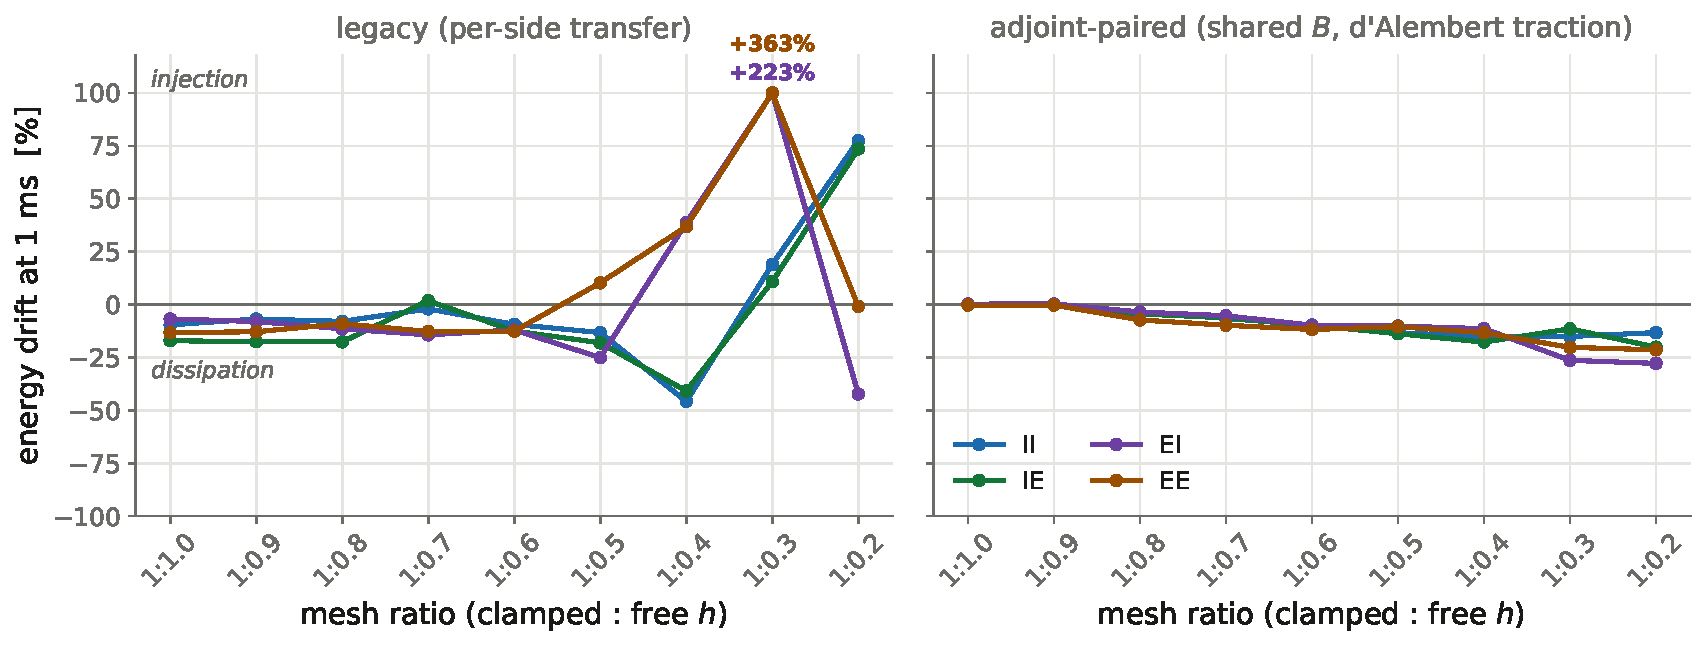
\includegraphics[width=\textwidth]{figs/legacy-vs-paired.pdf}
\caption{Non-overlap impedance Schwarz, energy drift at 1\,ms across the
mesh-ratio family, all four integrator combinations. Left: legacy per-side
transfer (consistent-mass integer-step metric) --- sign-indefinite, with
injection up to $+363\%$ (EE) and $+223\%$ (EI) at $1{:}0.3$. Right: the
adjoint-paired coupling (staggered lumped-mass metric of
Eq.~\eqref{eq:staggered} for explicit members) --- monotone, sign-definite
trace-jump dissipation at every ratio, and conservation to $\le 0.3\%$ on
conforming and $1{:}0.9$ meshes.}
\label{fig:legacy-paired}
\end{figure}

Three properties, in order of importance. First, \emph{no injection at any
ratio}: the interface work is sign-definite, as the telescoping identity
\eqref{eq:telescope} guarantees --- the wild $-53 \to +174 \to -66\%$ swings
of the overlap family and the $+363\%$ blowups of the legacy nonoverlap
coupling are gone. Second, near-conservation through mild contrast
($-0.03\%$ at $1{:}0.9$, where every other variant tested loses or gains
several percent). Third, the residual dissipation at strong contrast is the
\emph{genuine} trace-space jump being absorbed at the rate
$Z\!\int_\Gamma \jump{\dot{~u}}^2$: at the exactly nested ratio $1{:}0.5$
(where the legacy transfer is coincidentally adjoint and quadrature is
exact) paired and legacy agree to $0.1\%$, so the remaining loss is not a
transfer artifact but the Gander--Halpern--Nataf price of coupling trace
spaces that genuinely cannot represent each other's content --- now paid in
a controlled, monotone, sign-definite form.

\subsection{Explicit subdomains: IMEX interface treatment}
\label{sec:imex}

With an explicit (central-difference) subdomain on either side, the paired
coupling is violently unstable ($+10^3$ to $+10^5\,\%$) if the interface
terms are evaluated at lagged time levels: the consistent traction couples
the partner's \emph{acceleration} into the interface force, an algebraic
loop that the implicit pairs resolve within the Schwarz iteration. The cure
is the Phase~4 structure (Liu et al.'s IMEX-Newmark), now implemented:
because the dashpot force is linear in the unknown acceleration, the
explicit update is closed implicitly on the interface rows only,
\begin{equation}
  \bigl(~M + \gamma\,\Delta t\,Z\,W\bigr)\big|_\Gamma\, ~a_{n+1}
  \;=\; ~M\,~a^{\mathrm{expl}}\big|_\Gamma,
  \label{eq:imex}
\end{equation}
a small SPD solve per interface (reused for the three components) while the
interior stays matrix-free explicit; the dashpot then acts on the
end-of-step velocity $\dot{~u}_{n+1} = \tilde{~u} + \gamma\Delta t\,~a_{n+1}$
and the Schwarz iteration synchronizes both sides at $t_{n+1}$ exactly as in
the implicit--implicit case. Paired drift at 1\,ms, all combos:

\begin{center}
\begin{tabular}{lrrrr}
\toprule
ratio & II & IE & EI & EE \\
\midrule
1:1.0 & $-0.03$ & $-10.3$ & $-4.1$ & $-8.5$ \\
1:0.9 & $-0.03$ & $-8.2$ & $-4.5$ & $-9.4$ \\
1:0.8 & $-3.6$ & $-11.6$ & $-10.2$ & $-16.0$ \\
1:0.7 & $-6.6$ & $-15.9$ & $-12.2$ & $-19.0$ \\
1:0.6 & $-9.7$ & $-19.2$ & $-25.0$ & $-27.3$ \\
1:0.5 & $-13.3$ & $-21.2$ & $-21.0$ & $-24.9$ \\
1:0.4 & $-15.1$ & $-25.6$ & $-21.3$ & $-29.4$ \\
1:0.3 & $-15.1$ & $-21.6$ & $-33.8$ & $-37.2$ \\
1:0.2 & $-13.3$ & $-30.2$ & $-30.0$ & $-35.3$ \\
\bottomrule
\end{tabular}
\end{center}

Sign-definite everywhere: no injection at any ratio in any combination. The
explicit columns of this table must, however, be read against the right
reference: a \emph{monodomain} central-difference run of the same beam reads
$-8.2\%$ in the energy metric used here (consistent-mass kinetic energy
sampled at integer steps). Against that reference the conforming paired EE
run is exact to $0.35\%$ \emph{pointwise over the whole millisecond} --- the
coupled trajectory \emph{is} the monodomain trajectory, as the fixed-point
argument predicts.

\emph{Resolved: the $-8.2\%$ band was the metric, not the physics.} Central
difference advances the \emph{lumped}-mass system with leapfrog structure,
so the discrete energy it conserves exactly (linear problems) is the
staggered lumped-mass form
\begin{equation}
  E_n \;=\; \tfrac12\,\dot{~u}_{n-\frac12}^{T} ~M_L\, \dot{~u}_{n+\frac12}
        + \mathrm{SE}(~u_n)
      \;=\; \tfrac12\,\dot{~u}_n^{T} ~M_L\, \dot{~u}_n
        - \tfrac{\Delta t^2}{8}\, ~a_n^{T} ~M_L\, ~a_n
        + \mathrm{SE}(~u_n).
  \label{eq:staggered}
\end{equation}
Evaluating instead the consistent-mass integer-step kinetic energy
misprices the short-wavelength content of the sharp release front twice
over (consistent vs.\ lumped Rayleigh quotients diverge at high wavenumber,
and the integer-step velocity aliases the staggered content). The staggered
correction alone is $\Delta t$-dependent and small; the mass operator is
the dominant term --- which is why the band originally read as
``$\Delta t$-independent mesh dispersion.'' With the energy CSV evaluating
\eqref{eq:staggered} for central-difference subdomains (implemented in
\code{overlap\_energy.jl}), the monodomain explicit run conserves to
$\pm 0.000\%$ over the full millisecond, and the paired table becomes, at
1\,ms:

\begin{center}
\begin{tabular}{lrrrr}
\toprule
ratio & II & IE & EI & EE \\
\midrule
1:1.0 & $-0.03$ & $-0.11$ & $+0.20$ & $-0.27$ \\
1:0.9 & $-0.03$ & $-0.10$ & $+0.29$ & $-0.27$ \\
1:0.8 & $-3.6$ & $-4.4$ & $-3.5$ & $-7.3$ \\
1:0.7 & $-6.6$ & $-6.2$ & $-5.3$ & $-9.8$ \\
1:0.6 & $-9.7$ & $-9.8$ & $-9.8$ & $-11.8$ \\
1:0.5 & $-13.3$ & $-13.8$ & $-10.2$ & $-10.5$ \\
1:0.4 & $-15.1$ & $-17.8$ & $-11.4$ & $-13.3$ \\
1:0.3 & $-15.1$ & $-11.5$ & $-26.4$ & $-20.2$ \\
1:0.2 & $-13.3$ & $-20.1$ & $-27.8$ & $-21.4$ \\
\bottomrule
\end{tabular}
\end{center}

On conforming and mildly nonconforming meshes \emph{all four} integrator
combinations now conserve to $\le 0.3\%$; the nonconforming columns carry
the same monotone, sign-definite trace-jump dissipation in every
combination. (The tiny positive EI entries, $+0.2$--$0.3\%$, are bounded
transient storage in the conservative interface spring, not secular
growth.)

\subsection{Subcycled (multi-time-step) pairing}
\label{sec:subcycle}

Different time steps per subdomain require no new exchange machinery: each
subdomain records its per-substep trajectory (kinematics \emph{and}
internal force) during every Schwarz iteration, the coupling evaluates the
partner's state in time at each of its own substeps, and the paired
d'Alembert traction follows. (Enabling this exposed a time-step erosion bug
in the subcycler --- the stop-aligned remainder step persisted as the
nominal step and the Schwarz re-integration amplified the floating-point
remainder geometrically until the step collapsed --- fixed independently of
the pairing.)

The exchange was \emph{intended} to interpolate the partner
piecewise-linearly in time --- the interpolated-continuity structure under
which Gravouil--Combescure prove the subcycled interface work dissipative
($E_{\mathrm{int}} \le 0$, $O(\Delta t)$) --- but two infrastructure
defects, found while implementing the Prakash--Hjelmstad refinement below,
meant that is not what actually ran. First, the history interpolation
selected the wrong segment (an off-by-one that returned the end-of-history
value for any query in the last segment, and extrapolated backward off the
following segment elsewhere). Second, the per-stop history was anchored at
the \emph{first substep}, not the stop start, so a non-subcycling
partner's ``history'' was a single end-of-stop entry. Net effect: both
directions of the exchange end-sampled the partner's stop-end state ---
constant, not interpolated, data. With both defects fixed the exchange is
genuinely piecewise-linear in both directions. Drift at 1\,ms, free side
subcycled $4{:}1$ ($\Delta t = 0.25\,\mu$s inside the $1\,\mu$s stop,
clamped side at $1\,\mu$s; measured on one harness for all columns):

\begin{center}
\begin{tabular}{lrr}
\toprule
case & end-sampled (as shipped) & interpolated (GC, fixed) \\
\midrule
conforming II & $-2.8$ & $-3.6$ \\
conforming IE & $-9.6$ & $-10.1$ \\
conforming EE & $-10.6$ & $-9.6$ \\
1:0.5 II & $-20.6$ & $\mathbf{-14.1}$ \\
1:0.5 IE & $-24.4$ & $\mathbf{-21.3}$ \\
\bottomrule
\end{tabular}
\end{center}

(Both columns are measured in the consistent-mass integer-step metric for
comparability with the development history; in the staggered lumped-mass
metric of \eqref{eq:staggered} the shipped interpolated exchange reads
conforming II $-3.6$, IE $-1.4$, EE $-1.2$, and $1{:}0.5$ II $-14.1$,
IE $-14.3\%$ --- the explicit subcycled overhead is about one percent on
conforming meshes.) Genuine interpolation wins decisively at mesh contrast,
where end-sampling aliases the fine side's intra-window motion into the
exchanged traction ($-20.6 \to -14.1\%$). It \emph{loses} slightly on the conforming implicit
cases because the end-sampled datum is not merely aliased --- being the
stop-\emph{end} value applied throughout the window, it \emph{leads} the
true trajectory, and that anticipatory bias is a mild energy-injection
channel that happened to offset part of the GC dissipation. A cancellation
between two discretization crimes is not a conservation property, and it
collapses exactly where the stakes are high (strong contrast); the
interpolated exchange is now the behavior of the paired coupling.

\subsubsection*{The Prakash--Hjelmstad refinement is not partitioned-compatible}

Prakash--Hjelmstad telescope the subcycled interface work to exactly zero
by giving the interface traction a linear-in-time representation
$\hat\lambda(t)$ whose step values satisfy
$\tfrac12(\hat\lambda_n + \hat\lambda_{n+1}) = \overline{\lambda}_{n \to
n+1}$ (the partner's window average), so the trapezoidal work sums of the
two sides cancel window by window. Three Schwarz-compatible constructions
of this datum were implemented and measured on the benchmark above:

\begin{description}
  \item[Window average.] Handing the coarse side the partner's trapezoidal
  window average is work-conjugate to the fine side's interpolation ---
  but an average estimates the window \emph{midpoint}, and the half-window
  lag of the interface force behind the interface motion is artificial
  damping: uniformly worse than plain interpolation ($-3.6 \to -4.2$,
  $-10.1 \to -11.1$, $-9.6 \to -12.3$, $-14.1 \to -15.5$, $-21.3 \to
  -23.0$).
  \item[Exact telescoping recursion.] The de-lagged datum
  $\hat\lambda_{n+1} = 2\overline{\lambda} - \hat\lambda_n$ satisfies the
  telescoping identity exactly --- and diverges: the factor of two on the
  partner-state channel doubles the Schwarz fixed-point iteration's
  contraction factor, and the coupled iteration blows up within tens of
  stops.
  \item[Least-squares endpoint fit.] The endpoint value of the LS linear
  fit of the partner trajectory over the window is lag-free, filters
  intra-window content instead of aliasing it, and telescopes for
  window-linear tractions. It is stable over tens of stops and passes the
  short regression --- and over hundreds of stops it pumps energy
  catastrophically ($+10^3$--$10^5\%$ before aborting): a zero-lag
  filtered estimate is an extrapolation, and its frequency response
  exceeds unity off the linear band.
\end{description}

The pattern is the classical stability folklore of partitioned coupling:
only \emph{causal} transfer operators (lag $\ge 0$) are robust in a
fixed-point exchange, and every zero-lag work-conjugate datum is
anticipatory. Prakash--Hjelmstad's telescoping is consistent with this ---
their method solves the coupled interface problem \emph{directly} (a
FETI-style interface system per large step), which is precisely what a
partitioned Schwarz sweep does not do. Exact subcycled interface-work
telescoping therefore requires a direct interface solve, not a smarter
exchange; within the Schwarz family, genuinely interpolated GC transfer is
the measured stable optimum, and its $O(\Delta t)$ dissipation
($-3.6\%$ at conforming II vs.\ $-0.03\%$ same-step) is the price of
subcycling.

\section{The ten-millisecond horizon: long-time behavior}
\label{sec:tenms}

Every conclusion above rests on 1\,ms runs --- about two transits of the
release front. To test which behaviors are steady and which are transients,
all $151$ study configurations were re-run to $10$\,ms ($10^4$ stops at
$\Delta t = 10^{-6}$\,s): the full overlap sweep ($3$ widths $\times$ $9$
ratios $\times$ $4$ combos, fixed relaxation $\theta = 0.5$ as before), the
nonoverlap paired sweep and its subcycled set (now under
\code{relaxation: aitken recursive}), and fresh monodomain references. Two
validations anchor the data set: both monodomain references conserve the
staggered energy \eqref{eq:staggered} to $\pm 0.000\%$ over the full
$10$\,ms, and every surviving run reproduces its recorded 1\,ms drift at
its $t = 1$\,ms row --- for the nonoverlap runs this doubles as a
measurement that Aitken relaxation changes the iteration cost
($\approx 3\times$ fewer sweeps), not the fixed point.

\subsection*{Overlap: the 1\,ms drifts were transients of instabilities}

The overlap family is long-horizon unstable almost everywhere. Of the
$108$ overlap runs, $74$ died of element inversion after exponential
energy growth (typically $+3{,}000$ to $+10{,}000\%$ of $E_0$ at death,
between $2$ and $9$\,ms), and most of the remainder collapsed toward zero
energy instead. The sign-indefinite $\pm$tens-of-percent drifts of the
1\,ms sweep (Sec.~\ref{sec:ratiosweep}) were early sections of these
trajectories: configurations that read as ``dissipative'' at 1\,ms (e.g.\
maximum overlap $1{:}0.6$ II, $-61\%$) reversed and blew up ($+5{,}432\%$
at death). Mesh conformity does not save the mixed-integrator combos: the
conforming half-overlap IE run read $+13\%$ at 1\,ms, grew cleanly
exponentially ($\times 3.3$ at $4$\,ms, $\times 38$ at $6$\,ms), and died
at $6.25$\,ms; conforming EI behaves alike at all three widths. The only
healthy overlap configurations at $10$\,ms are the conforming II runs:
$+0.64$, $+0.61$, $+0.16\%$ at overlap widths $0.0508$, $0.0254$,
$0.0127$\,m. The overlap coupling is therefore a short-horizon method on
nonconforming meshes, and for non-II combos even on conforming ones
(Fig.~\ref{fig:overlap-10ms}).

\begin{figure}[htbp]
\centering
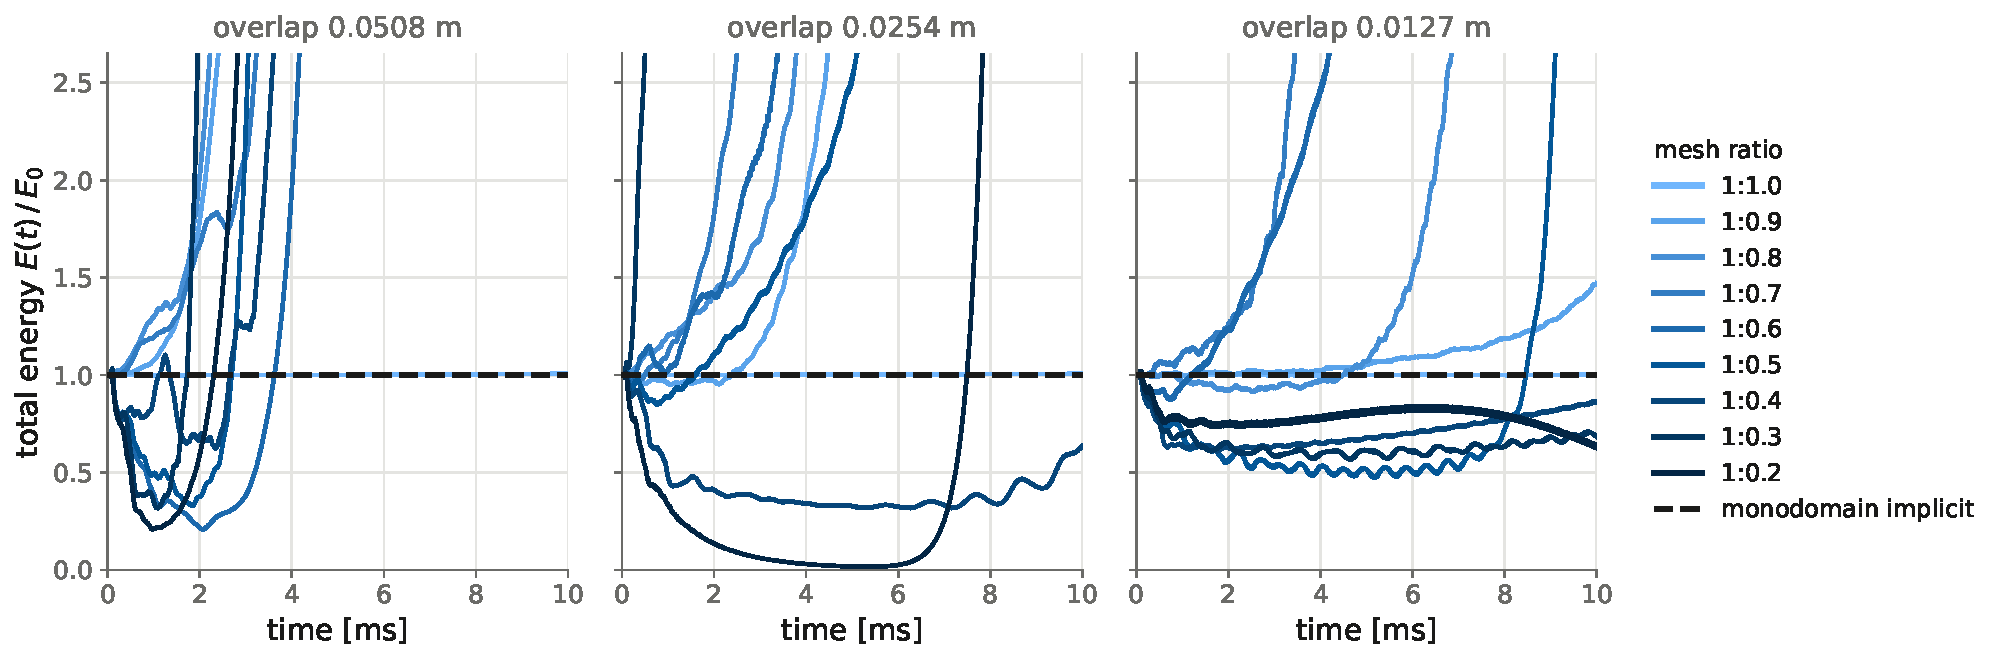
\includegraphics[width=\textwidth]{figs/overlap-II-10ms.pdf}
\caption{Overlap impedance Schwarz (variational transfer),
implicit--implicit, $10$\,ms horizon. Nearly every nonconforming
configuration either grows exponentially until element inversion kills the
run (curves leaving the top of the axes) or collapses toward zero energy;
only the conforming ($1{:}1.0$) runs track the monodomain reference. The
mixed and all-explicit combinations (not shown) are worse: they lose even
the conforming cases.}
\label{fig:overlap-10ms}
\end{figure}

\subsection*{Nonoverlap pairing: no injection, but the dissipation
compounds --- and two new failure modes appear}

The paired nonoverlap coupling never injects at any ratio in any
combination, at $10$\,ms as at $1$\,ms. Its monotone trace-jump
dissipation, however, compounds. Drift at $10$\,ms ($\dagger\,t$ marks a
run dead by element inversion at $t$\,ms; EE entries marked $\ast$ ended
in the noise-saturated state discussed below):

\begin{center}
\begin{tabular}{lrrrr}
\toprule
ratio & II & IE & EI & EE \\
\midrule
1:1.0 & $+0.00$ & $-0.9$ & $-0.2$ & $\ast$ \\
1:0.9 & $+0.00$ & $-0.5$ & $+0.1$ & $\ast$ \\
1:0.8 & $\dagger\,5.2$ & $\dagger\,3.9$ & $\dagger\,4.0$ & $\dagger\,2.6$ \\
1:0.7 & $\dagger\,4.9$ & $\dagger\,3.7$ & $\dagger\,3.9$ & $\dagger\,2.8$ \\
1:0.6 & $-47.3$ & $-56.4$ & $-42.9$ & $\ast$ \\
1:0.5 & $-56.8$ & $-72.0$ & $-40.8$ & $\ast$ \\
1:0.4 & $-54.9$ & $-73.9$ & $-40.4$ & $\ast$ \\
1:0.3 & $-65.1$ & $-66.0$ & $-81.1$ & $\ast$ \\
1:0.2 & $-53.3$ & $-73.1$ & $-84.1$ & $\ast$ \\
\bottomrule
\end{tabular}
\end{center}

\begin{figure}[htbp]
\centering
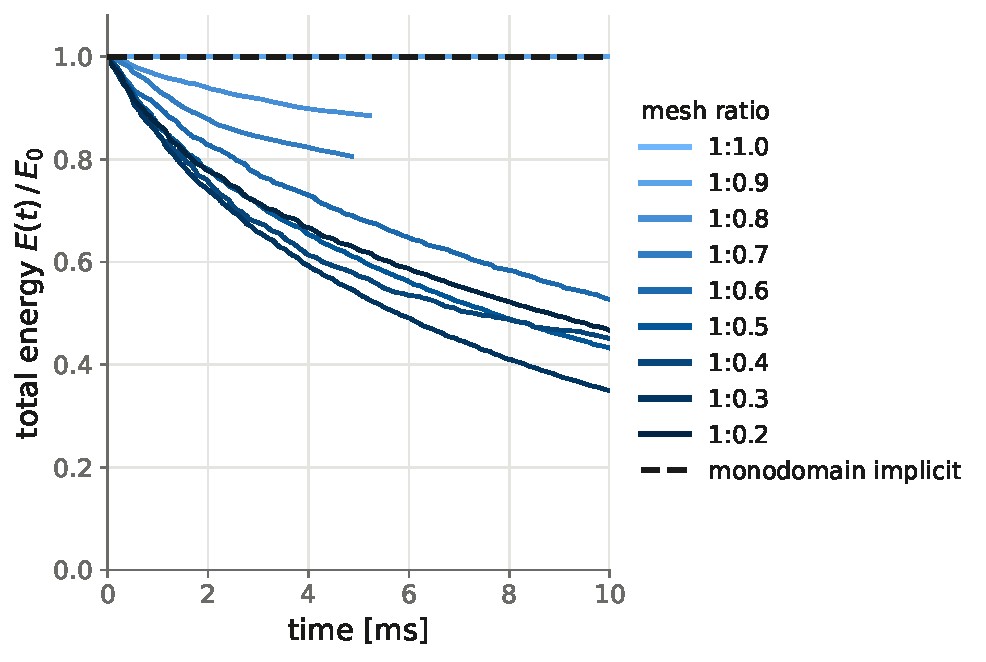
\includegraphics[width=0.495\textwidth]{figs/nonoverlap-II-10ms.pdf}\hfill
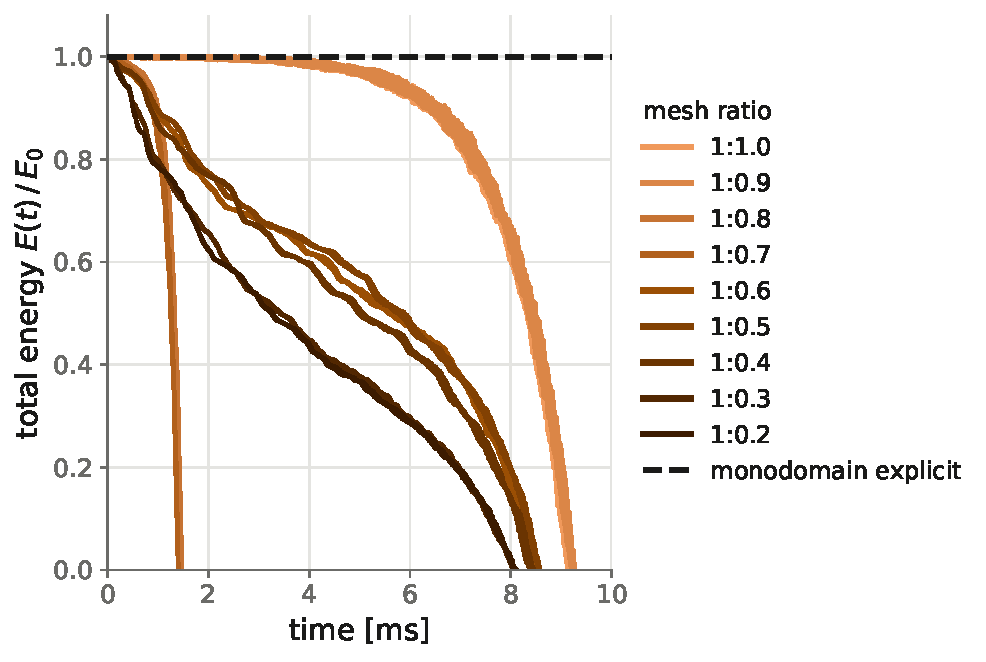
\includegraphics[width=0.495\textwidth]{figs/nonoverlap-EE-10ms.pdf}
\caption{Adjoint-paired nonoverlap impedance Schwarz, $10$\,ms horizon,
staggered energy metric. Left: implicit--implicit --- no injection
anywhere; conforming and $1{:}0.9$ hold the monodomain reference, strong
contrast dissipates monotonically, and the non-nested ratios
$1{:}0.7$--$1{:}0.8$ end early at $\approx 5$\,ms (interface element
inversion). Right: explicit--explicit --- the staggered kinetic term goes
secularly negative at every ratio as undamped grid-frequency content
accumulates at $\mathrm{CFL}=1$; the $1{:}0.7$--$1{:}0.8$ runs die of
central-difference instability at $2.6$--$2.8$\,ms.}
\label{fig:nonoverlap-10ms}
\end{figure}

Three observations (Fig.~\ref{fig:nonoverlap-10ms}, left). First, the
conforming and $1{:}0.9$ columns with an
implicit member are outstanding --- the coupling holds $0.00$ to $-0.9\%$
over ten thousand stops. Second, at strong contrast ($\le 1{:}0.6$) the
sign-definite dissipation that read as $10$--$28\%$ at 1\,ms reaches
$40$--$85\%$ by $10$\,ms: bounded and ordered, but far too large for
wave-transit accuracy. Absorption of unrepresentable content is a rate,
not a one-time toll.

Third, the mildly nonconforming, \emph{non-nested} ratios $1{:}0.7$ and
$1{:}0.8$ form a failure window invisible at 1\,ms: the paired transfer
accumulates interface-local high-frequency displacement content, and every
integrator combination eventually dies there --- explicit members at
$2.6$--$4$\,ms by central-difference instability, implicit pairs at
$\approx 5$\,ms when the first interface element inverts while the
\emph{global} energy is still smooth and healthy ($-19\%$ at death). This
is not an Aitken artifact: re-runs with fixed $\theta = 0.5$ die
identically (II $1{:}0.7$ at $5.15$ vs.\ $4.86$\,ms, trajectories matching
to three digits), so the noise accumulation belongs to the transfer
operators themselves. The nested ratios ($1{:}0.5$ exactly, and the strong
ratios whose transfer filters aggressively) do not exhibit it.

\subsection*{Explicit--explicit saturation, and subcycling as a remedy}

The EE column degrades at \emph{every} ratio by $10$\,ms, conforming
included (Fig.~\ref{fig:nonoverlap-10ms}, right), ending with the
staggered metric near $-2\,E_0$. The end state
is not a blow-up: the stored energy stays bounded and physical throughout
(the conforming run holds $E/E_0 \ge 0.97$ to $5$\,ms, then slides), but
the staggered kinetic term goes steadily negative --- the signature of
sawtooth content at $\omega\Delta t \approx 2$ accumulating in velocity
and acceleration. Central difference at $\mathrm{CFL} = 1$ has zero
numerical dissipation at the stability edge, so whatever grid-frequency
content the interface exchange seeds is never removed; with no implicit
member in the pair, it accumulates without bound in amplitude-neutral
modes. The measured remedy is time-step margin: the \emph{subcycled}
conforming EE run (free side at $\Delta t/4$, $\mathrm{CFL} = 0.25$) ends
at $-10.8\%$ with no saturation. Subcycling cuts the other way for II:
the same-step conforming II run conserves to $+0.00\%$ while the subcycled
one loses $-20.2\%$ (at $1{:}0.5$, $-61.6\%$) --- the
Gravouil--Combescure interpolation dissipation of
Sec.~\ref{sec:subcycle}, harmless per stop, compounds over $10^4$ stops.
At long horizons the multi-time-step exchange is thus a trade: it
stabilizes explicit members (CFL margin) and taxes implicit ones
(interpolation dissipation). Figure~\ref{fig:subcycled-10ms} shows both
sides of the trade on one axis.

\begin{figure}[htbp]
\centering
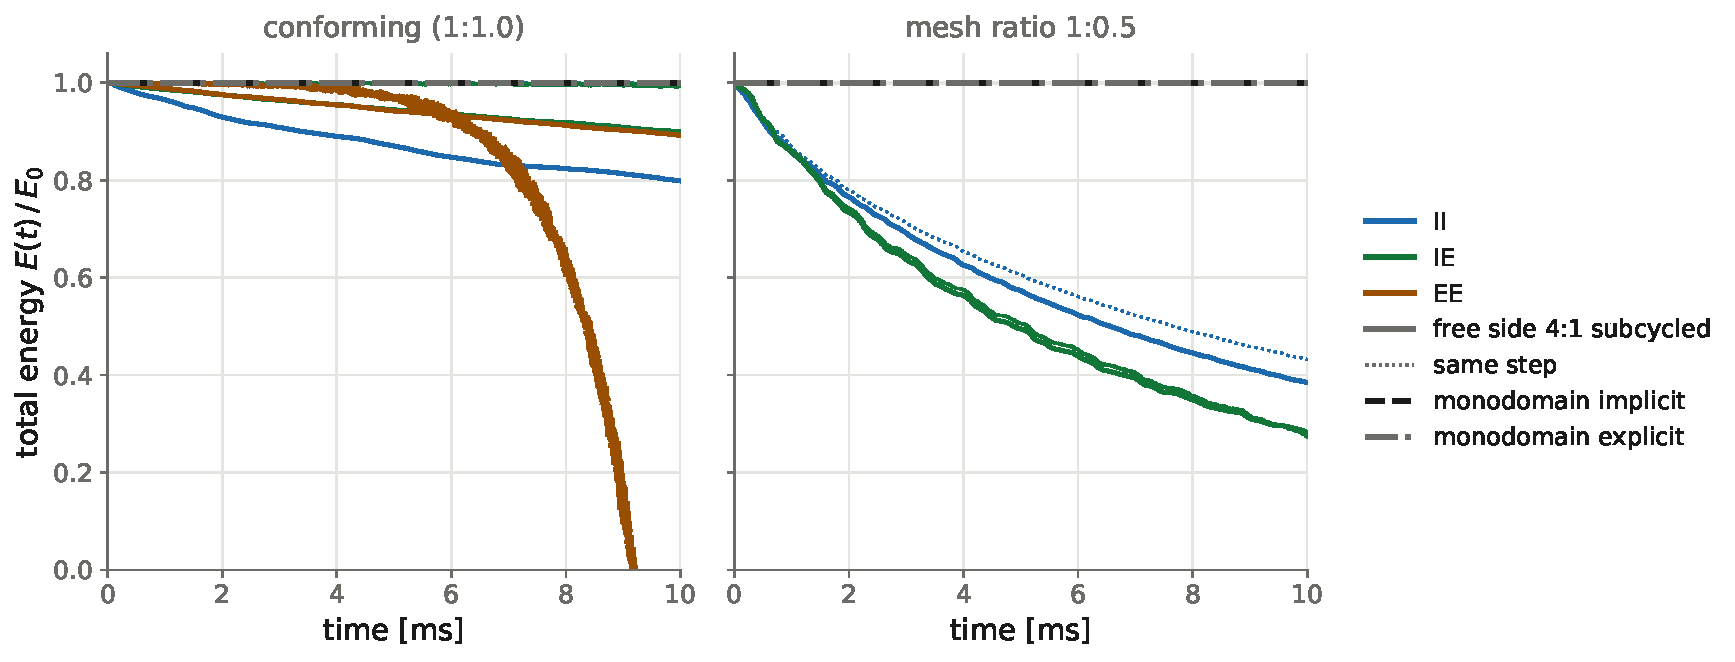
\includegraphics[width=\textwidth]{figs/nonoverlap-subcycled-10ms.pdf}
\caption{Subcycled (free side $4{:}1$, solid) vs same-step (dotted)
adjoint-paired nonoverlap coupling over $10$\,ms. Left, conforming: the
subcycled EE run (orange solid, $\mathrm{CFL}=0.25$) avoids the saturation
that destroys same-step EE (orange dotted), while subcycled II (blue
solid) pays the compounding Gravouil--Combescure interpolation dissipation
that same-step II (on the reference line) does not. Right, mesh ratio
$1{:}0.5$: at strong contrast the trace-jump dissipation dominates and the
subcycling overhead is comparatively small (II subcycled $-61.6\%$ vs
same-step $-56.8\%$).}
\label{fig:subcycled-10ms}
\end{figure}

The long-horizon ranking is unambiguous: adjoint-paired nonoverlap
coupling with at least one implicit interface member, on conforming or
nested mesh ratios, is the only tested configuration that is sound at
$10$\,ms; the overlap family is short-horizon only. Data, figures, and the
run harness: \code{\textasciitilde/cantilever-energy-study/}
(\code{*-10ms} data directories, \code{wccm-plots/*-10ms}, and
\code{drift-table-10ms.txt}).

\section{Windowed controller stops: the relaxation state must be
slot-keyed}
\label{sec:windowed}

The multi-domain controller advances in \emph{stops}; within a stop each
subdomain subcycles to the stop end with its own time step, and partner
data are exchanged as per-substep trajectories with piecewise-linear time
interpolation (Sec.~\ref{sec:subcycle}). This raises a configuration
question the study had not yet touched: with the subdomain steps held
fixed ($1\,\mu$s), does the \emph{controller} stop size --- the
``window'' over which the Schwarz iteration converges before committing
--- affect the converged physics? A sweep over windows of $1$ (baseline),
$2$, $5$, and $10\,\mu$s on representative overlap and nonoverlap cases,
run to $10$\,ms, gave a split answer. (Data:
\code{controller-step-sweep/} in the study bundle.)

\textbf{Overlap: a pure cost knob.} Every overlap trajectory is identical
across all four windows to all printed digits --- the conforming II run
ends at $+0.61\%$ in all four, and the $1{:}0.5$ instability even dies at
the same instant ($7.25$--$7.26$\,ms). The overlap exchange interpolates
partner kinematics from history with no per-pair relaxation state, so the
windowed waveform iteration converges to the same-step fixed point.

\textbf{Nonoverlap: the window shifted the fixed point.} Drift for the
conforming paired II case at $10$\,ms: $+0.00\%$ same-step, $+11.3\%$ at
the $2\,\mu$s window, $-81.9\%$ at $5\,\mu$s, $-83.7\%$ at $10\,\mu$s
(Aitken relaxation; with fixed $\theta = 0.5$ the sequence is a monotone
drain instead, $-7.1\%$ at $2\,\mu$s to $-87.9\%$ at $10\,\mu$s). This
was not a convergence failure --- the sweeps converged normally --- but a
defect of the relaxation machinery: the relaxation state
($\lambda$ vectors and Aitken residual buffers) was stored as \emph{one
vector per interface pair}, updated on every BC application. In a
windowed stop the relaxed side of a pair (the later-listed member)
applies its coupling BC once per \emph{substep}, so the blend
$(1-\theta)\,g + \theta\,\mathrm{rhs}$ mixed iterates across \emph{time}
rather than across Schwarz sweeps: a causal exponential low-pass (lag
$\sim \Delta t_{\mathrm{sub}}/\theta$) on the exchanged traction, whose
lag dissipation grows with the window. Under Aitken the defect changes
sign: the $\theta$ estimate compares residuals belonging to different
times, overshoots past $1$, and the resulting phase \emph{lead} injects
energy --- the $+11.3\%$ entry. (The subcycled study of
Sec.~\ref{sec:subcycle} escaped by an ordering accident: its subcycling
free side is listed first, i.e.\ unrelaxed.)

Two experiments isolate and confirm the mechanism. First, $\theta = 1$
--- which uses no relaxation state at all --- reproduces the same-step
physics on the \emph{unmodified} code at every window ($+0.00\%$ over
the full $10$\,ms at the $10\,\mu$s window; the EE case recovers its
same-step saturation exactly). Second, with the fix below in place, all
windowed policies land on the same-step trajectory. The fix keys the
relaxation state by pair \emph{and} by substep time slot within the
current stop, clearing it at every stop; with one substep per stop it
reduces exactly to the classical per-pair iteration, and the same-step
code path is bit-identical to the pre-fix baselines. Windowed runs then
match same-step to Schwarz truncation (the residual $3.9\times 10^{-6}$
displacement mismatch at working tolerances collapses to
$3.7\times 10^{-8}$ as the stopping tolerances tighten), and a
windowed-equivalence regression now guards this in the adjoint-pairing
test.

\begin{figure}[htbp]
\centering
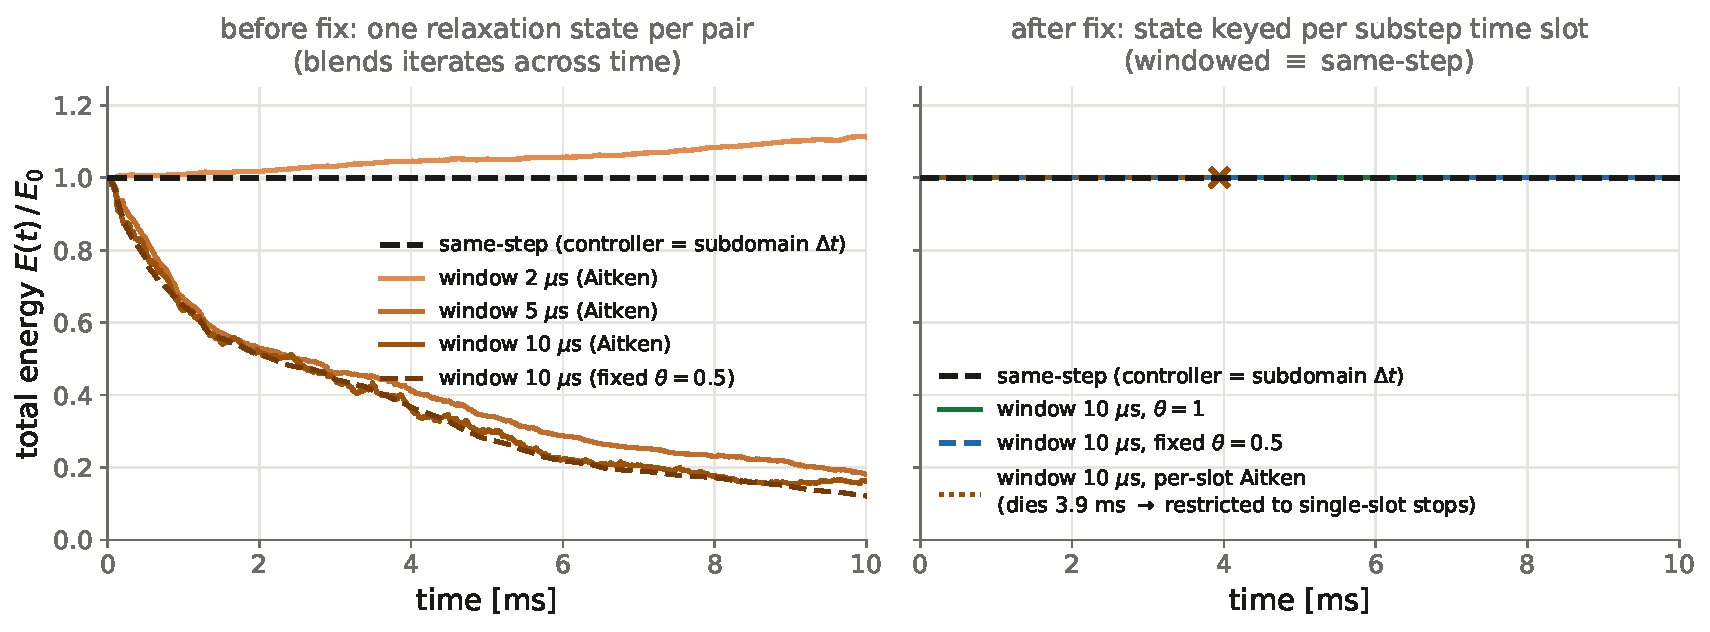
\includegraphics[width=\textwidth]{figs/windowed-stops.pdf}
\caption{Windowed controller stops on the conforming paired II case,
$10$\,ms. Left, pre-fix: the per-pair relaxation state blends iterates
across time --- Aitken injects at the $2\,\mu$s window and drains at
$5$--$10\,\mu$s; fixed $\theta = 0.5$ drains monotonically. Right,
post-fix (slot-keyed state): every windowed policy lands on the same-step
trajectory; the per-slot Aitken run is physically correct until its
unclamped $\theta$ excursions kill the Newton solve at $3.9$\,ms
($\times$), which motivated restricting Aitken to single-slot stops.}
\label{fig:windowed}
\end{figure}

\textbf{Relaxation policy inside windows.} With the state fixed, the
remaining question is which relaxation policy a windowed stop should use.
Measured on the conforming II case at the $10\,\mu$s window (mean Schwarz
sweeps per stop): $\theta = 1$ converges in $19.1$ and runs the full
$10$\,ms cleanly; per-slot Aitken takes ${\sim}25$ and dies at $3.9$\,ms
when an unclamped $\theta$ excursion feeds the Newton solve a divergent
iterate; fixed $\theta = 0.5$ takes $47.5$ (clean); and a waveform-pooled
Aitken (one $\theta$ from residuals pooled across the window's slots)
takes $55.1$ --- clean on II but fatal on EE, where it locks $\theta$
persistently negative. Aitken acceleration is therefore at best useless
and at worst fatal inside windows, and Norma now applies it only to
single-slot stops, where its ${\approx}3\times$ sweep reduction is
proven; windowed stops use the configured relaxation parameter, with
$\theta = 1$ recommended --- the impedance dashpot supplies the
contraction, so no under-relaxation is needed.

Two limitations round out the picture. The all-explicit pair at large
windows is impractical under \emph{any} policy: the windowed explicit
sweep map is nearly non-contractive (fixed $\theta = 0.5$ rides the
$128$-sweep cap and still dies at $9.8$\,ms). And windows are never a
cost optimization for the nonoverlap exchange: the number of substep
solves per unit time is (sweeps per stop)$/\Delta t_{\mathrm{sub}}$
regardless of the window, and the windowed sweep counts above all exceed
the same-step Aitken count, so the controller step is purely a
convenience knob (e.g.\ aligning output stops), cost-neutral at best.
For the overlap family, by contrast, larger stops are a mild speedup
(fewer, barely-more-iterated stops). One earlier observation is
withdrawn as an artifact: the pre-fix ``EE at the $2\,\mu$s window with
fixed $\theta$ ends at $-0.25\%$'' entry was the defect's low-pass
accidentally damping the grid-frequency saturation; post-fix, windowed
EE saturates exactly like same-step EE, and the honest remedy remains
CFL margin via subcycling (Sec.~\ref{sec:tenms}).

\textbf{Open issue: a $\theta$-sensitive fixed point.} The
windowed-equivalence test exposed a pre-existing defect, orthogonal to
the fix: the \emph{converged} paired-impedance solution depends weakly on
the relaxation parameter --- $\theta = 0.5$ and $\theta = 1.0$ differ by
${\sim}4\times 10^{-5}$ relative displacement on the $2{:}1$
nonconforming cantilever at a $10^{-13}$ stopping tolerance, same-step
and windowed alike, and an Aitken run lands on the $\theta = 1$ answer to
$10^{-12}$. Instrumentation rules out the blend algebra (the blended
``base'' is identically zero at interface DOFs, because
\code{apply\_bcs} zeroes the boundary force before each pass); the
evidence points to a neutral --- non-contracting --- mode of the paired
exchange that retains its $\theta$-dependent initialization and is
invisible to the displacement-based stopping criterion. The magnitude is
far below every signal in this study ($\ge 10^{-4}$), but it is a genuine
correctness question and needs its own investigation.

\section{Where this lands}
\label{sec:conclusion}

For wave-transit problems on \emph{nonconforming overlapping} decompositions,
the tested coupling family is absorbing-or-unstable: hard Dirichlet matching
(pointwise or weak) is violently unstable, and the impedance condition is
stable precisely because its dashpot continually absorbs the inter-grid
disagreement, whose dominant component is coarse-grid dispersion --- a smooth,
in-band solution defect that neither spatial filtering (Phase~2, falsified)
nor transfer improvements (Phase~1) can close at fixed $h$. The ratio sweep
(Sec.~\ref{sec:ratiosweep}) removes the remaining comfort: the interface work
is sign-indefinite in practice as well as in principle, so the ``price'' is
not a bounded, predictable dissipation --- neighboring mesh ratios swing from
$-53\%$ to $+174\%$ to $-66\%$. The ten-millisecond horizon
(Sec.~\ref{sec:tenms}) removes the last of it: those swings are early
sections of exponential instabilities, $74$ of the $108$ overlap runs die
of element inversion by $9$\,ms, and even conforming meshes only save the
implicit--implicit combination. Mesh conformity \emph{and} implicit
integration on both sides therefore remain the only route to long-horizon
energy conservation within the overlap family; everything else is usable
for short transients at most, with the channel-resolved instrumentation
reporting the damage.

For energy-critical nonconforming coupling, the theory-backed path --- the
\emph{nonoverlap} impedance variant, whose single shared interface admits the
adjoint pairing \eqref{eq:adjoint} --- is now implemented and validated
(Sec.~\ref{sec:nonoverlap}): with the consistent d'Alembert traction and the
paired operators, implicit--implicit coupling conserves to $-0.03\%$ through
mild mesh contrast and degrades into monotone, sign-definite, bounded
dissipation at strong contrast, with no injection anywhere. Explicit
subdomains are covered by the IMEX interface treatment
(Sec.~\ref{sec:imex}): the conforming explicit--explicit trajectory matches
the monodomain explicit run to $0.35\%$ pointwise, and every combination is
sign-definite at every ratio. The ten-millisecond study
(Sec.~\ref{sec:tenms}) qualifies this in three ways: the paired
dissipation at strong contrast is a rate that compounds to $40$--$85\%$
over $10^4$ stops; the mild non-nested ratios $1{:}0.7$--$1{:}0.8$
accumulate interface-local high-frequency content until an interface
element inverts (all combinations, implicit included, $2.6$--$5$\,ms);
and the all-explicit pair at $\mathrm{CFL}=1$ saturates with undamped
grid-frequency content at every ratio, for which time-step margin
(measured via the subcycled free side at $\mathrm{CFL}=0.25$) is an
effective remedy. The practical recommendation is therefore:
conforming meshes within the overlap family (implicit--implicit only for
long horizons), or the adjoint-paired
nonoverlap variant (now the default for \code{Schwarz impedance nonoverlap}; \code{adjoint pairing: false} restores the legacy transfer) with at least
one implicit interface member and a conforming or nested mesh ratio when
the decomposition
must be nonconforming and the energy budget matters. Subcycled
(multi-time-step) pairing is validated with genuinely interpolated
Gravouil--Combescure transfer --- two infrastructure defects that had
silently reduced it to end-sampling are fixed, halving the excess
dissipation at strong mesh contrast (Sec.~\ref{sec:subcycle}). The
Prakash--Hjelmstad exact-telescoping refinement was implemented in three
Schwarz-compatible forms and measured to be structurally incompatible with
a partitioned exchange (lagged forms over-dissipate; zero-lag forms are
anticipatory and unstable); realizing it requires a direct FETI-style
interface solve per large step, which, together with the
localized-Lagrange-multiplier frame construction (Park--Felippa; Dvorak et
al.\ 2023), remains follow-up work. Finally, the Schwarz controller step is
now a pure convenience knob for both families: the relaxation-state defect
that made windowed stops shift the nonoverlap fixed point is fixed
(slot-keyed state; windowed $\equiv$ same-step to Schwarz truncation), with
Aitken acceleration restricted to the single-slot stops where it provably
helps (Sec.~\ref{sec:windowed}). The one open correctness question left by
that investigation is the weakly $\theta$-sensitive fixed point of the
paired exchange (${\sim}4\times 10^{-5}$ relative displacement), evidence
of a neutral mode invisible to the displacement-based stopping criterion.

\end{document}
